\documentclass[1p]{elsarticle_modified}
%\bibliographystyle{elsarticle-num}

%\usepackage[colorlinks]{hyperref}
%\usepackage{abbrmath_seonhwa} %\Abb, \Ascr, \Acal ,\Abf, \Afrak
\usepackage{amsfonts}
\usepackage{amssymb}
\usepackage{amsmath}
\usepackage{amsthm}
\usepackage{scalefnt}
\usepackage{amsbsy}
\usepackage{kotex}
\usepackage{caption}
\usepackage{subfig}
\usepackage{color}
\usepackage{graphicx}
\usepackage{xcolor} %% white, black, red, green, blue, cyan, magenta, yellow
\usepackage{float}
\usepackage{setspace}
\usepackage{hyperref}

\usepackage{tikz}
\usetikzlibrary{arrows}

\usepackage{multirow}
\usepackage{array} % fixed length table
\usepackage{hhline}

%%%%%%%%%%%%%%%%%%%%%
\makeatletter
\renewcommand*\env@matrix[1][\arraystretch]{%
	\edef\arraystretch{#1}%
	\hskip -\arraycolsep
	\let\@ifnextchar\new@ifnextchar
	\array{*\c@MaxMatrixCols c}}
\makeatother %https://tex.stackexchange.com/questions/14071/how-can-i-increase-the-line-spacing-in-a-matrix
%%%%%%%%%%%%%%%

\usepackage[normalem]{ulem}

\newcommand{\msout}[1]{\ifmmode\text{\sout{\ensuremath{#1}}}\else\sout{#1}\fi}
%SOURCE: \msout is \stkout macro in https://tex.stackexchange.com/questions/20609/strikeout-in-math-mode

\newcommand{\cancel}[1]{
	\ifmmode
	{\color{red}\msout{#1}}
	\else
	{\color{red}\sout{#1}}
	\fi
}

\newcommand{\add}[1]{
	{\color{blue}\uwave{#1}}
}

\newcommand{\replace}[2]{
	\ifmmode
	{\color{red}\msout{#1}}{\color{blue}\uwave{#2}}
	\else
	{\color{red}\sout{#1}}{\color{blue}\uwave{#2}}
	\fi
}

\newcommand{\Sol}{\mathcal{S}} %segment
\newcommand{\D}{D} %diagram
\newcommand{\A}{\mathcal{A}} %arc


%%%%%%%%%%%%%%%%%%%%%%%%%%%%%5 test

\def\sl{\operatorname{\textup{SL}}(2,\Cbb)}
\def\psl{\operatorname{\textup{PSL}}(2,\Cbb)}
\def\quan{\mkern 1mu \triangleright \mkern 1mu}

\theoremstyle{definition}
\newtheorem{thm}{Theorem}[section]
\newtheorem{prop}[thm]{Proposition}
\newtheorem{lem}[thm]{Lemma}
\newtheorem{ques}[thm]{Question}
\newtheorem{cor}[thm]{Corollary}
\newtheorem{defn}[thm]{Definition}
\newtheorem{exam}[thm]{Example}
\newtheorem{rmk}[thm]{Remark}
\newtheorem{alg}[thm]{Algorithm}

\newcommand{\I}{\sqrt{-1}}
\begin{document}

%\begin{frontmatter}
%
%\title{Boundary parabolic representations of knots up to 8 crossings}
%
%%% Group authors per affiliation:
%\author{Yunhi Cho} 
%\address{Department of Mathematics, University of Seoul, Seoul, Korea}
%\ead{yhcho@uos.ac.kr}
%
%
%\author{Seonhwa Kim} %\fnref{s_kim}}
%\address{Center for Geometry and Physics, Institute for Basic Science, Pohang, 37673, Korea}
%\ead{ryeona17@ibs.re.kr}
%
%\author{Hyuk Kim}
%\address{Department of Mathematical Sciences, Seoul National University, Seoul 08826, Korea}
%\ead{hyukkim@snu.ac.kr}
%
%\author{Seokbeom Yoon}
%\address{Department of Mathematical Sciences, Seoul National University, Seoul, 08826,  Korea}
%\ead{sbyoon15@snu.ac.kr}
%
%\begin{abstract}
%We find all boundary parabolic representation of knots up to 8 crossings.
%
%\end{abstract}
%\begin{keyword}
%    \MSC[2010] 57M25 
%\end{keyword}
%
%\end{frontmatter}

%\linenumbers
%\tableofcontents
%
\newcommand\colored[1]{\textcolor{white}{\rule[-0.35ex]{0.8em}{1.4ex}}\kern-0.8em\color{red} #1}%
%\newcommand\colored[1]{\textcolor{white}{ #1}\kern-2.17ex	\textcolor{white}{ #1}\kern-1.81ex	\textcolor{white}{ #1}\kern-2.15ex\color{red}#1	}

{\Large $\underline{12n_{0789}~(K12n_{0789})}$}

\setlength{\tabcolsep}{10pt}
\renewcommand{\arraystretch}{1.6}
\vspace{1cm}\begin{tabular}{m{100pt}>{\centering\arraybackslash}m{274pt}}
\multirow{5}{120pt}{
	\centering
	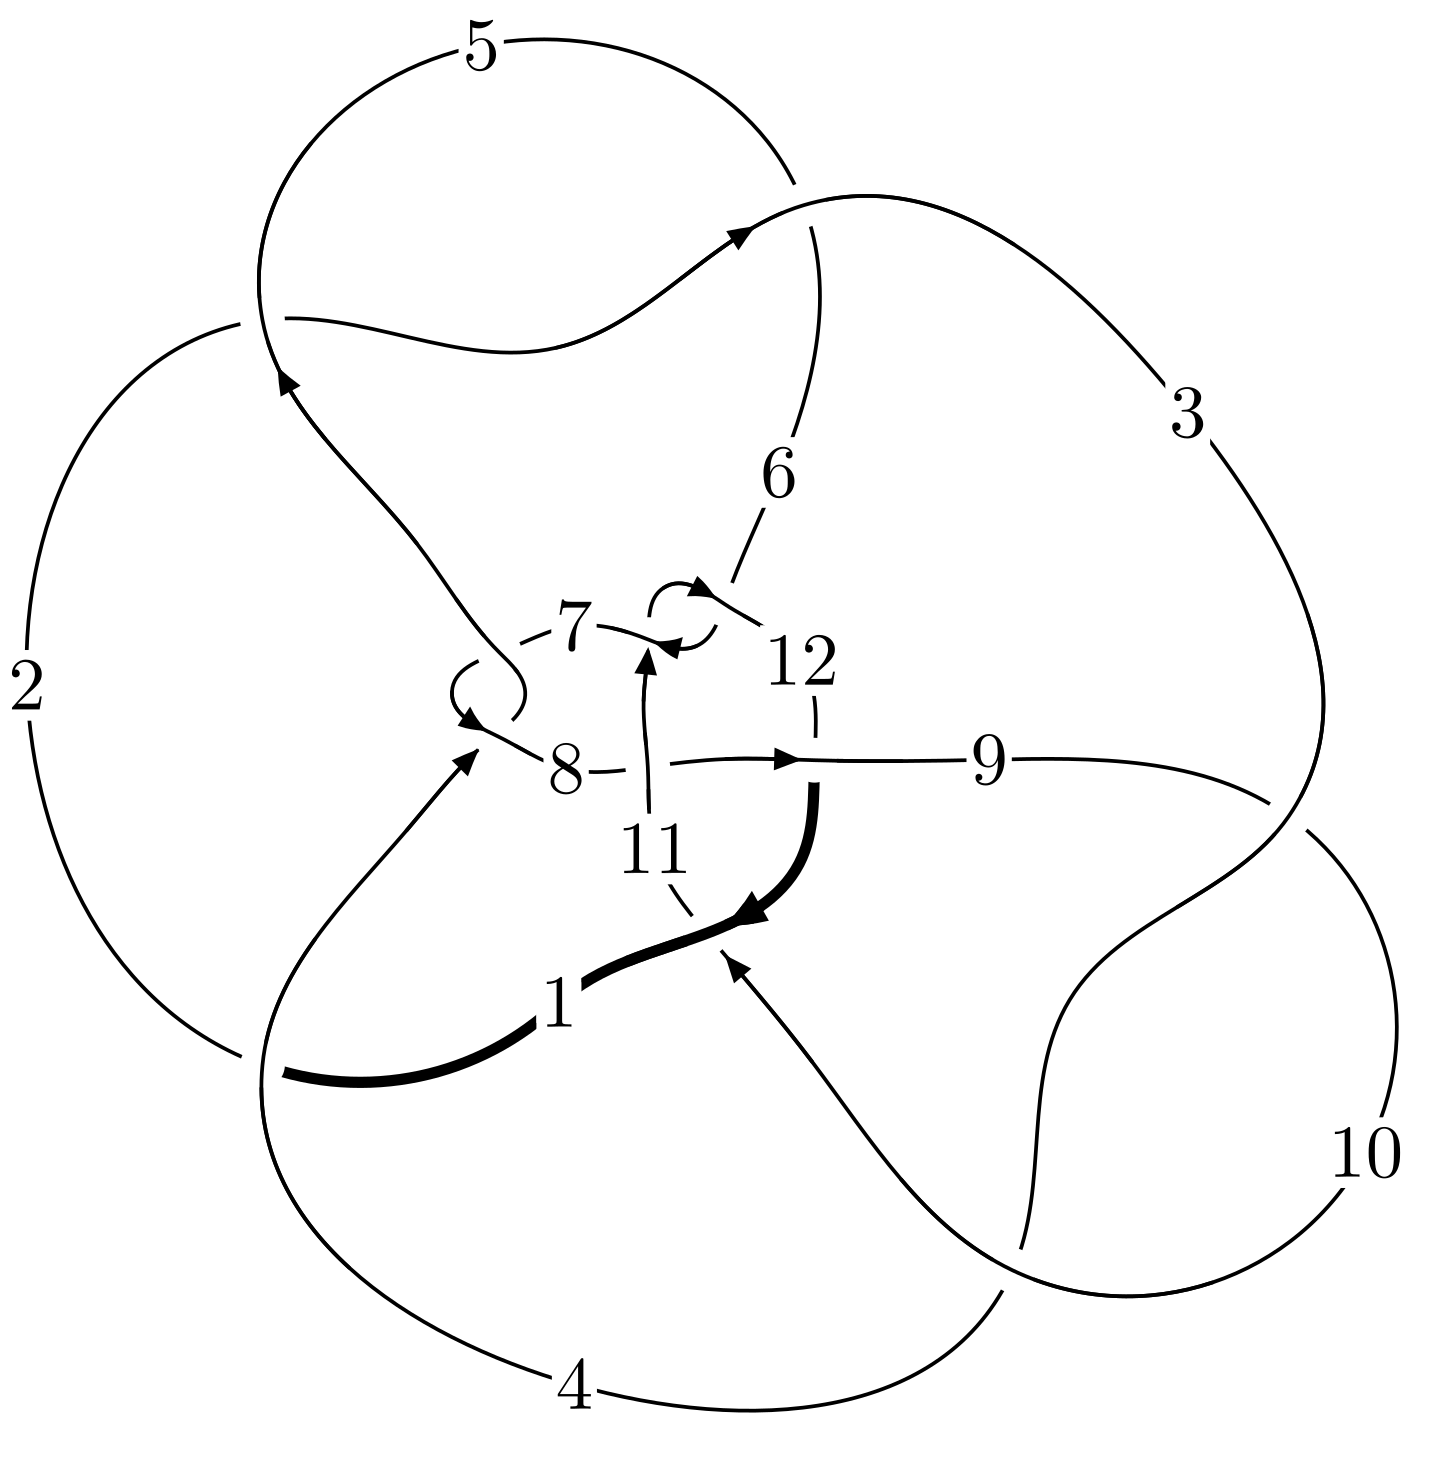
\includegraphics[width=112pt]{../../../GIT/diagram.site/Diagrams/png/2878_12n_0789.png}\\
\ \ \ A knot diagram\footnotemark}&
\allowdisplaybreaks
\textbf{Linearized knot diagam} \\
\cline{2-2}
 &
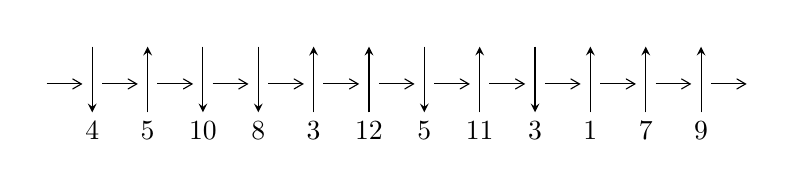
\begin{tikzpicture}[x=20pt, y=17pt]
	% nodes
	\node (C0) at (0, 0) {};
	\node (C1) at (1, 0) {};
	\node (C1U) at (1, +1) {};
	\node (C1D) at (1, -1) {4};

	\node (C2) at (2, 0) {};
	\node (C2U) at (2, +1) {};
	\node (C2D) at (2, -1) {5};

	\node (C3) at (3, 0) {};
	\node (C3U) at (3, +1) {};
	\node (C3D) at (3, -1) {10};

	\node (C4) at (4, 0) {};
	\node (C4U) at (4, +1) {};
	\node (C4D) at (4, -1) {8};

	\node (C5) at (5, 0) {};
	\node (C5U) at (5, +1) {};
	\node (C5D) at (5, -1) {3};

	\node (C6) at (6, 0) {};
	\node (C6U) at (6, +1) {};
	\node (C6D) at (6, -1) {12};

	\node (C7) at (7, 0) {};
	\node (C7U) at (7, +1) {};
	\node (C7D) at (7, -1) {5};

	\node (C8) at (8, 0) {};
	\node (C8U) at (8, +1) {};
	\node (C8D) at (8, -1) {11};

	\node (C9) at (9, 0) {};
	\node (C9U) at (9, +1) {};
	\node (C9D) at (9, -1) {3};

	\node (C10) at (10, 0) {};
	\node (C10U) at (10, +1) {};
	\node (C10D) at (10, -1) {1};

	\node (C11) at (11, 0) {};
	\node (C11U) at (11, +1) {};
	\node (C11D) at (11, -1) {7};

	\node (C12) at (12, 0) {};
	\node (C12U) at (12, +1) {};
	\node (C12D) at (12, -1) {9};
	\node (C13) at (13, 0) {};

	% arrows
	\draw[->,>={angle 60}]
	(C0) edge (C1) (C1) edge (C2) (C2) edge (C3) (C3) edge (C4) (C4) edge (C5) (C5) edge (C6) (C6) edge (C7) (C7) edge (C8) (C8) edge (C9) (C9) edge (C10) (C10) edge (C11) (C11) edge (C12) (C12) edge (C13) ;	\draw[->,>=stealth]
	(C1U) edge (C1D) (C2D) edge (C2U) (C3U) edge (C3D) (C4U) edge (C4D) (C5D) edge (C5U) (C6D) edge (C6U) (C7U) edge (C7D) (C8D) edge (C8U) (C9U) edge (C9D) (C10D) edge (C10U) (C11D) edge (C11U) (C12D) edge (C12U) ;
	\end{tikzpicture} \\
\hhline{~~} \\& 
\textbf{Solving Sequence} \\ \cline{2-2} 
 &
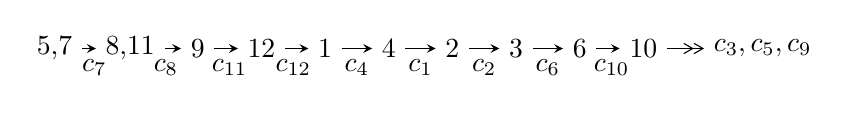
\begin{tikzpicture}[x=23pt, y=7pt]
	% node
	\node (A0) at (-1/8, 0) {5,7};
	\node (A1) at (17/16, 0) {8,11};
	\node (A2) at (17/8, 0) {9};
	\node (A3) at (25/8, 0) {12};
	\node (A4) at (33/8, 0) {1};
	\node (A5) at (41/8, 0) {4};
	\node (A6) at (49/8, 0) {2};
	\node (A7) at (57/8, 0) {3};
	\node (A8) at (65/8, 0) {6};
	\node (A9) at (73/8, 0) {10};
	\node (C1) at (1/2, -1) {$c_{7}$};
	\node (C2) at (13/8, -1) {$c_{8}$};
	\node (C3) at (21/8, -1) {$c_{11}$};
	\node (C4) at (29/8, -1) {$c_{12}$};
	\node (C5) at (37/8, -1) {$c_{4}$};
	\node (C6) at (45/8, -1) {$c_{1}$};
	\node (C7) at (53/8, -1) {$c_{2}$};
	\node (C8) at (61/8, -1) {$c_{6}$};
	\node (C9) at (69/8, -1) {$c_{10}$};
	\node (A10) at (11, 0) {$c_{3},c_{5},c_{9}$};

	% edge
	\draw[->,>=stealth]	
	(A0) edge (A1) (A1) edge (A2) (A2) edge (A3) (A3) edge (A4) (A4) edge (A5) (A5) edge (A6) (A6) edge (A7) (A7) edge (A8) (A8) edge (A9) ;
	\draw[->>,>={angle 60}]	
	(A9) edge (A10);
\end{tikzpicture} \\ 

\end{tabular} \\

\footnotetext{
The image of knot diagram is generated by the software ``\textbf{Draw programme}" developed by Andrew Bartholomew(\url{http://www.layer8.co.uk/maths/draw/index.htm\#Running-draw}), where we modified some parts for our purpose(\url{https://github.com/CATsTAILs/LinksPainter}).
}\phantom \\ \newline 
\centering \textbf{Ideals for irreducible components\footnotemark of $X_{\text{par}}$} 
 
\begin{align*}
I^u_{1}&=\langle 
-9.62341\times10^{256} u^{81}+4.36659\times10^{257} u^{80}+\cdots+3.22941\times10^{256} b-7.42547\times10^{256},\\
\phantom{I^u_{1}}&\phantom{= \langle  }4.79036\times10^{256} u^{81}-4.33578\times10^{257} u^{80}+\cdots+3.22941\times10^{256} a-1.08341\times10^{258},\;u^{82}-5 u^{81}+\cdots-9 u+1\rangle \\
I^u_{2}&=\langle 
-2.14857\times10^{33} u^{37}-1.68774\times10^{34} u^{36}+\cdots+4.97146\times10^{32} b-1.06077\times10^{33},\\
\phantom{I^u_{2}}&\phantom{= \langle  }3.40194\times10^{33} u^{37}+2.65994\times10^{34} u^{36}+\cdots+4.97146\times10^{32} a+3.48145\times10^{33},\;u^{38}+8 u^{37}+\cdots+7 u+1\rangle \\
\\
\end{align*}
\raggedright * 2 irreducible components of $\dim_{\mathbb{C}}=0$, with total 120 representations.\\
\footnotetext{All coefficients of polynomials are rational numbers. But the coefficients are sometimes approximated in decimal forms when there is not enough margin.}
\newpage
\renewcommand{\arraystretch}{1}
\centering \section*{I. $I^u_{1}= \langle -9.62\times10^{256} u^{81}+4.37\times10^{257} u^{80}+\cdots+3.23\times10^{256} b-7.43\times10^{256},\;4.79\times10^{256} u^{81}-4.34\times10^{257} u^{80}+\cdots+3.23\times10^{256} a-1.08\times10^{258},\;u^{82}-5 u^{81}+\cdots-9 u+1 \rangle$}
\flushleft \textbf{(i) Arc colorings}\\
\begin{tabular}{m{7pt} m{180pt} m{7pt} m{180pt} }
\flushright $a_{5}=$&$\begin{pmatrix}0\\u\end{pmatrix}$ \\
\flushright $a_{7}=$&$\begin{pmatrix}1\\0\end{pmatrix}$ \\
\flushright $a_{8}=$&$\begin{pmatrix}1\\u^2\end{pmatrix}$ \\
\flushright $a_{11}=$&$\begin{pmatrix}-1.48335 u^{81}+13.4259 u^{80}+\cdots-314.049 u+33.5482\\2.97993 u^{81}-13.5213 u^{80}+\cdots+0.624686 u+2.29933\end{pmatrix}$ \\
\flushright $a_{9}=$&$\begin{pmatrix}-6.90787 u^{81}+34.0673 u^{80}+\cdots-7.25907 u-12.3927\\-3.93969 u^{81}+21.1683 u^{80}+\cdots-134.630 u+16.2614\end{pmatrix}$ \\
\flushright $a_{12}=$&$\begin{pmatrix}1.49657 u^{81}-0.0953944 u^{80}+\cdots-313.424 u+35.8475\\2.97993 u^{81}-13.5213 u^{80}+\cdots+0.624686 u+2.29933\end{pmatrix}$ \\
\flushright $a_{1}=$&$\begin{pmatrix}-6.98693 u^{81}+29.0151 u^{80}+\cdots+266.633 u-50.5502\\-5.97289 u^{81}+28.6846 u^{80}+\cdots-19.3508 u-3.05047\end{pmatrix}$ \\
\flushright $a_{4}=$&$\begin{pmatrix}u\\u^3+u\end{pmatrix}$ \\
\flushright $a_{2}=$&$\begin{pmatrix}-8.09243 u^{81}+34.6437 u^{80}+\cdots+228.950 u-46.1752\\-6.93732 u^{81}+33.6383 u^{80}+\cdots-55.0188 u+1.22337\end{pmatrix}$ \\
\flushright $a_{3}=$&$\begin{pmatrix}-8.09243 u^{81}+34.6437 u^{80}+\cdots+228.950 u-46.1752\\-6.40134 u^{81}+30.5632 u^{80}+\cdots-10.7452 u-4.59507\end{pmatrix}$ \\
\flushright $a_{6}=$&$\begin{pmatrix}18.4534 u^{81}-92.4177 u^{80}+\cdots+301.801 u-21.4321\\2.22211 u^{81}-13.2729 u^{80}+\cdots+136.502 u-18.2729\end{pmatrix}$ \\
\flushright $a_{10}=$&$\begin{pmatrix}-1.54299 u^{81}+11.0282 u^{80}+\cdots-136.510 u+14.2742\\2.49596 u^{81}-11.4503 u^{80}+\cdots+53.5123 u-3.37749\end{pmatrix}$\\&\end{tabular}
\flushleft \textbf{(ii) Obstruction class $= -1$}\\~\\
\flushleft \textbf{(iii) Cusp Shapes $= -2.97826 u^{81}+10.7782 u^{80}+\cdots+181.549 u-52.6251$}\\~\\
\newpage\renewcommand{\arraystretch}{1}
\flushleft \textbf{(iv) u-Polynomials at the component}\newline \\
\begin{tabular}{m{50pt}|m{274pt}}
Crossings & \hspace{64pt}u-Polynomials at each crossing \\
\hline $$\begin{aligned}c_{1}\end{aligned}$$&$\begin{aligned}
&u^{82}-2 u^{81}+\cdots-144006814 u+92506631
\end{aligned}$\\
\hline $$\begin{aligned}c_{2},c_{5}\end{aligned}$$&$\begin{aligned}
&u^{82}+8 u^{81}+\cdots+285305320 u+28654393
\end{aligned}$\\
\hline $$\begin{aligned}c_{3},c_{9}\end{aligned}$$&$\begin{aligned}
&u^{82}-2 u^{81}+\cdots+3176 u+3053
\end{aligned}$\\
\hline $$\begin{aligned}c_{4},c_{7}\end{aligned}$$&$\begin{aligned}
&u^{82}-5 u^{81}+\cdots-9 u+1
\end{aligned}$\\
\hline $$\begin{aligned}c_{6},c_{11}\end{aligned}$$&$\begin{aligned}
&u^{82}-2 u^{81}+\cdots-1903 u+193
\end{aligned}$\\
\hline $$\begin{aligned}c_{8}\end{aligned}$$&$\begin{aligned}
&u^{82}+3 u^{81}+\cdots-14399 u+1273
\end{aligned}$\\
\hline $$\begin{aligned}c_{10}\end{aligned}$$&$\begin{aligned}
&u^{82}+4 u^{81}+\cdots+1322 u+307
\end{aligned}$\\
\hline $$\begin{aligned}c_{12}\end{aligned}$$&$\begin{aligned}
&u^{82}-4 u^{81}+\cdots-360727464 u+76941877
\end{aligned}$\\
\hline
\end{tabular}\\~\\
\newpage\renewcommand{\arraystretch}{1}
\flushleft \textbf{(v) Riley Polynomials at the component}\newline \\
\begin{tabular}{m{50pt}|m{274pt}}
Crossings & \hspace{64pt}Riley Polynomials at each crossing \\
\hline $$\begin{aligned}c_{1}\end{aligned}$$&$\begin{aligned}
&y^{82}-86 y^{81}+\cdots-27578920347511596 y+8557476778970161
\end{aligned}$\\
\hline $$\begin{aligned}c_{2},c_{5}\end{aligned}$$&$\begin{aligned}
&y^{82}+84 y^{81}+\cdots-16527381541916668 y+821074238198449
\end{aligned}$\\
\hline $$\begin{aligned}c_{3},c_{9}\end{aligned}$$&$\begin{aligned}
&y^{82}-70 y^{81}+\cdots-64668510 y+9320809
\end{aligned}$\\
\hline $$\begin{aligned}c_{4},c_{7}\end{aligned}$$&$\begin{aligned}
&y^{82}+19 y^{81}+\cdots+81 y+1
\end{aligned}$\\
\hline $$\begin{aligned}c_{6},c_{11}\end{aligned}$$&$\begin{aligned}
&y^{82}+76 y^{81}+\cdots-3045 y+37249
\end{aligned}$\\
\hline $$\begin{aligned}c_{8}\end{aligned}$$&$\begin{aligned}
&y^{82}+19 y^{81}+\cdots+35322967 y+1620529
\end{aligned}$\\
\hline $$\begin{aligned}c_{10}\end{aligned}$$&$\begin{aligned}
&y^{82}+4 y^{81}+\cdots+789978 y+94249
\end{aligned}$\\
\hline $$\begin{aligned}c_{12}\end{aligned}$$&$\begin{aligned}
&y^{82}+38 y^{81}+\cdots+86506044299292766 y+5920052436283129
\end{aligned}$\\
\hline
\end{tabular}\\~\\
\newpage\flushleft \textbf{(vi) Complex Volumes and Cusp Shapes}
$$\begin{array}{c|c|c}  
\text{Solutions to }I^u_{1}& \I (\text{vol} + \sqrt{-1}CS) & \text{Cusp shape}\\
 \hline 
\begin{aligned}
u &= \phantom{-}0.056723 + 0.964872 I \\
a &= \phantom{-}1.37031 + 0.67536 I \\
b &= -0.289704 - 0.025564 I\end{aligned}
 & \phantom{-}1.40440 + 4.15567 I & \phantom{-0.000000 } 0 \\ \hline\begin{aligned}
u &= \phantom{-}0.056723 - 0.964872 I \\
a &= \phantom{-}1.37031 - 0.67536 I \\
b &= -0.289704 + 0.025564 I\end{aligned}
 & \phantom{-}1.40440 - 4.15567 I & \phantom{-0.000000 } 0 \\ \hline\begin{aligned}
u &= -0.178708 + 1.060670 I \\
a &= \phantom{-}0.672194 - 0.146847 I \\
b &= -0.14351 - 1.65591 I\end{aligned}
 & -4.60976 - 1.70624 I & \phantom{-0.000000 } 0 \\ \hline\begin{aligned}
u &= -0.178708 - 1.060670 I \\
a &= \phantom{-}0.672194 + 0.146847 I \\
b &= -0.14351 + 1.65591 I\end{aligned}
 & -4.60976 + 1.70624 I & \phantom{-0.000000 } 0 \\ \hline\begin{aligned}
u &= -0.462793 + 0.789203 I \\
a &= \phantom{-}1.94590 + 0.72997 I \\
b &= -0.383521 - 1.052400 I\end{aligned}
 & -0.66968 + 1.34659 I & \phantom{-0.000000 } 0 \\ \hline\begin{aligned}
u &= -0.462793 - 0.789203 I \\
a &= \phantom{-}1.94590 - 0.72997 I \\
b &= -0.383521 + 1.052400 I\end{aligned}
 & -0.66968 - 1.34659 I & \phantom{-0.000000 } 0 \\ \hline\begin{aligned}
u &= -0.100143 + 0.905993 I \\
a &= -2.03793 + 0.42379 I \\
b &= \phantom{-}0.613296 + 0.753156 I\end{aligned}
 & \phantom{-}3.23144 - 0.92093 I & \phantom{-0.000000 } 0 \\ \hline\begin{aligned}
u &= -0.100143 - 0.905993 I \\
a &= -2.03793 - 0.42379 I \\
b &= \phantom{-}0.613296 - 0.753156 I\end{aligned}
 & \phantom{-}3.23144 + 0.92093 I & \phantom{-0.000000 } 0 \\ \hline\begin{aligned}
u &= \phantom{-}0.819623 + 0.726122 I \\
a &= \phantom{-}0.365501 + 0.230418 I \\
b &= \phantom{-}0.20556 + 1.48772 I\end{aligned}
 & -7.23484 - 0.77529 I & \phantom{-0.000000 } 0 \\ \hline\begin{aligned}
u &= \phantom{-}0.819623 - 0.726122 I \\
a &= \phantom{-}0.365501 - 0.230418 I \\
b &= \phantom{-}0.20556 - 1.48772 I\end{aligned}
 & -7.23484 + 0.77529 I & \phantom{-0.000000 } 0\\
 \hline 
 \end{array}$$\newpage$$\begin{array}{c|c|c}  
\text{Solutions to }I^u_{1}& \I (\text{vol} + \sqrt{-1}CS) & \text{Cusp shape}\\
 \hline 
\begin{aligned}
u &= \phantom{-}0.303048 + 0.851736 I \\
a &= -1.88227 - 1.10824 I \\
b &= \phantom{-}1.226900 - 0.082101 I\end{aligned}
 & \phantom{-}4.36049 - 2.15843 I & \phantom{-0.000000 } 0 \\ \hline\begin{aligned}
u &= \phantom{-}0.303048 - 0.851736 I \\
a &= -1.88227 + 1.10824 I \\
b &= \phantom{-}1.226900 + 0.082101 I\end{aligned}
 & \phantom{-}4.36049 + 2.15843 I & \phantom{-0.000000 } 0 \\ \hline\begin{aligned}
u &= \phantom{-}0.096694 + 1.151330 I \\
a &= \phantom{-}1.317440 - 0.057645 I \\
b &= -0.898102 - 0.440443 I\end{aligned}
 & \phantom{-}0.102335 - 0.805883 I & \phantom{-0.000000 } 0 \\ \hline\begin{aligned}
u &= \phantom{-}0.096694 - 1.151330 I \\
a &= \phantom{-}1.317440 + 0.057645 I \\
b &= -0.898102 + 0.440443 I\end{aligned}
 & \phantom{-}0.102335 + 0.805883 I & \phantom{-0.000000 } 0 \\ \hline\begin{aligned}
u &= -0.699295 + 0.395601 I \\
a &= \phantom{-}3.21229 - 2.97384 I \\
b &= \phantom{-}0.10447 - 1.70528 I\end{aligned}
 & -7.31286 + 5.25289 I & -4.83806 - 7.69489 I \\ \hline\begin{aligned}
u &= -0.699295 - 0.395601 I \\
a &= \phantom{-}3.21229 + 2.97384 I \\
b &= \phantom{-}0.10447 + 1.70528 I\end{aligned}
 & -7.31286 - 5.25289 I & -4.83806 + 7.69489 I \\ \hline\begin{aligned}
u &= \phantom{-}0.578459 + 0.528250 I \\
a &= \phantom{-}1.13288 + 1.69205 I \\
b &= \phantom{-}0.089527 + 0.178860 I\end{aligned}
 & -0.57429 - 6.85107 I & \phantom{-}2.69108 - 1.63480 I \\ \hline\begin{aligned}
u &= \phantom{-}0.578459 - 0.528250 I \\
a &= \phantom{-}1.13288 - 1.69205 I \\
b &= \phantom{-}0.089527 - 0.178860 I\end{aligned}
 & -0.57429 + 6.85107 I & \phantom{-}2.69108 + 1.63480 I \\ \hline\begin{aligned}
u &= -0.726408 + 0.292025 I \\
a &= \phantom{-}0.290860 + 0.066462 I \\
b &= -0.087141 - 1.137640 I\end{aligned}
 & -2.39617 + 2.63265 I & \phantom{-0.000000 } 0. - 3.56398 I \\ \hline\begin{aligned}
u &= -0.726408 - 0.292025 I \\
a &= \phantom{-}0.290860 - 0.066462 I \\
b &= -0.087141 + 1.137640 I\end{aligned}
 & -2.39617 - 2.63265 I & \phantom{-0.000000 -}0. + 3.56398 I\\
 \hline 
 \end{array}$$\newpage$$\begin{array}{c|c|c}  
\text{Solutions to }I^u_{1}& \I (\text{vol} + \sqrt{-1}CS) & \text{Cusp shape}\\
 \hline 
\begin{aligned}
u &= -0.389609 + 0.672619 I \\
a &= -0.312060 - 0.644701 I \\
b &= -0.10406 + 1.55102 I\end{aligned}
 & -5.28113 + 6.02668 I & -0.83509 - 9.93765 I \\ \hline\begin{aligned}
u &= -0.389609 - 0.672619 I \\
a &= -0.312060 + 0.644701 I \\
b &= -0.10406 - 1.55102 I\end{aligned}
 & -5.28113 - 6.02668 I & -0.83509 + 9.93765 I \\ \hline\begin{aligned}
u &= -1.227010 + 0.083228 I \\
a &= -0.228622 - 0.202291 I \\
b &= \phantom{-}0.125008 - 1.085830 I\end{aligned}
 & -6.76066 + 0.17831 I & \phantom{-0.000000 } 0 \\ \hline\begin{aligned}
u &= -1.227010 - 0.083228 I \\
a &= -0.228622 + 0.202291 I \\
b &= \phantom{-}0.125008 + 1.085830 I\end{aligned}
 & -6.76066 - 0.17831 I & \phantom{-0.000000 } 0 \\ \hline\begin{aligned}
u &= \phantom{-}0.213840 + 0.716879 I \\
a &= \phantom{-}2.94719 - 3.15470 I \\
b &= -0.10463 + 1.62106 I\end{aligned}
 & -4.77668 - 4.91554 I & \phantom{-}5.80425 + 7.31495 I \\ \hline\begin{aligned}
u &= \phantom{-}0.213840 - 0.716879 I \\
a &= \phantom{-}2.94719 + 3.15470 I \\
b &= -0.10463 - 1.62106 I\end{aligned}
 & -4.77668 + 4.91554 I & \phantom{-}5.80425 - 7.31495 I \\ \hline\begin{aligned}
u &= -0.845531 + 0.931008 I \\
a &= -0.790053 + 0.732156 I \\
b &= \phantom{-}0.887959 + 0.172806 I\end{aligned}
 & -2.10266 + 4.70360 I & \phantom{-0.000000 } 0 \\ \hline\begin{aligned}
u &= -0.845531 - 0.931008 I \\
a &= -0.790053 - 0.732156 I \\
b &= \phantom{-}0.887959 - 0.172806 I\end{aligned}
 & -2.10266 - 4.70360 I & \phantom{-0.000000 } 0 \\ \hline\begin{aligned}
u &= \phantom{-}0.749079 + 1.025990 I \\
a &= \phantom{-}1.47656 + 0.10493 I \\
b &= -0.27067 + 1.41969 I\end{aligned}
 & -6.33650 - 5.10935 I & \phantom{-0.000000 } 0 \\ \hline\begin{aligned}
u &= \phantom{-}0.749079 - 1.025990 I \\
a &= \phantom{-}1.47656 - 0.10493 I \\
b &= -0.27067 - 1.41969 I\end{aligned}
 & -6.33650 + 5.10935 I & \phantom{-0.000000 } 0\\
 \hline 
 \end{array}$$\newpage$$\begin{array}{c|c|c}  
\text{Solutions to }I^u_{1}& \I (\text{vol} + \sqrt{-1}CS) & \text{Cusp shape}\\
 \hline 
\begin{aligned}
u &= -0.646385 + 1.094070 I \\
a &= -1.088150 - 0.099223 I \\
b &= \phantom{-}0.582063 + 0.903467 I\end{aligned}
 & -3.13677 + 5.80187 I & \phantom{-0.000000 } 0 \\ \hline\begin{aligned}
u &= -0.646385 - 1.094070 I \\
a &= -1.088150 + 0.099223 I \\
b &= \phantom{-}0.582063 - 0.903467 I\end{aligned}
 & -3.13677 - 5.80187 I & \phantom{-0.000000 } 0 \\ \hline\begin{aligned}
u &= -0.862329 + 0.934321 I \\
a &= \phantom{-}0.528921 - 0.207487 I \\
b &= -0.651249 + 0.150043 I\end{aligned}
 & -2.11824 + 1.66557 I & \phantom{-0.000000 } 0 \\ \hline\begin{aligned}
u &= -0.862329 - 0.934321 I \\
a &= \phantom{-}0.528921 + 0.207487 I \\
b &= -0.651249 - 0.150043 I\end{aligned}
 & -2.11824 - 1.66557 I & \phantom{-0.000000 } 0 \\ \hline\begin{aligned}
u &= -0.366398 + 1.230750 I \\
a &= -1.44997 - 0.60149 I \\
b &= \phantom{-}0.645386 + 1.088180 I\end{aligned}
 & \phantom{-}2.07065 + 5.92091 I & \phantom{-0.000000 } 0 \\ \hline\begin{aligned}
u &= -0.366398 - 1.230750 I \\
a &= -1.44997 + 0.60149 I \\
b &= \phantom{-}0.645386 - 1.088180 I\end{aligned}
 & \phantom{-}2.07065 - 5.92091 I & \phantom{-0.000000 } 0 \\ \hline\begin{aligned}
u &= \phantom{-}0.542418 + 0.448908 I \\
a &= -0.808272 - 0.209146 I \\
b &= \phantom{-}0.410061 + 0.391443 I\end{aligned}
 & -2.49574 - 1.83560 I & \phantom{-}0.724028 + 0.349432 I \\ \hline\begin{aligned}
u &= \phantom{-}0.542418 - 0.448908 I \\
a &= -0.808272 + 0.209146 I \\
b &= \phantom{-}0.410061 - 0.391443 I\end{aligned}
 & -2.49574 + 1.83560 I & \phantom{-}0.724028 - 0.349432 I \\ \hline\begin{aligned}
u &= \phantom{-}0.962244 + 0.895870 I \\
a &= -1.59591 - 0.91749 I \\
b &= \phantom{-}0.86805 - 1.72981 I\end{aligned}
 & -13.1403 - 7.5526 I & \phantom{-0.000000 } 0 \\ \hline\begin{aligned}
u &= \phantom{-}0.962244 - 0.895870 I \\
a &= -1.59591 + 0.91749 I \\
b &= \phantom{-}0.86805 + 1.72981 I\end{aligned}
 & -13.1403 + 7.5526 I & \phantom{-0.000000 } 0\\
 \hline 
 \end{array}$$\newpage$$\begin{array}{c|c|c}  
\text{Solutions to }I^u_{1}& \I (\text{vol} + \sqrt{-1}CS) & \text{Cusp shape}\\
 \hline 
\begin{aligned}
u &= -1.069690 + 0.791365 I \\
a &= -0.263944 + 0.770014 I \\
b &= \phantom{-}1.58821 - 0.26194 I\end{aligned}
 & -8.81768 - 1.56510 I & \phantom{-0.000000 } 0 \\ \hline\begin{aligned}
u &= -1.069690 - 0.791365 I \\
a &= -0.263944 - 0.770014 I \\
b &= \phantom{-}1.58821 + 0.26194 I\end{aligned}
 & -8.81768 + 1.56510 I & \phantom{-0.000000 } 0 \\ \hline\begin{aligned}
u &= \phantom{-}0.880487 + 1.028230 I \\
a &= -0.277301 + 0.180815 I \\
b &= -0.80666 - 1.79638 I\end{aligned}
 & -12.69480 + 0.72849 I & \phantom{-0.000000 } 0 \\ \hline\begin{aligned}
u &= \phantom{-}0.880487 - 1.028230 I \\
a &= -0.277301 - 0.180815 I \\
b &= -0.80666 + 1.79638 I\end{aligned}
 & -12.69480 - 0.72849 I & \phantom{-0.000000 } 0 \\ \hline\begin{aligned}
u &= -0.353207 + 0.522372 I \\
a &= \phantom{-}0.740973 - 0.001919 I \\
b &= -0.218396 - 0.458164 I\end{aligned}
 & \phantom{-}0.013980 + 1.160290 I & \phantom{-}0.33727 - 6.21213 I \\ \hline\begin{aligned}
u &= -0.353207 - 0.522372 I \\
a &= \phantom{-}0.740973 + 0.001919 I \\
b &= -0.218396 + 0.458164 I\end{aligned}
 & \phantom{-}0.013980 - 1.160290 I & \phantom{-}0.33727 + 6.21213 I \\ \hline\begin{aligned}
u &= \phantom{-}1.159320 + 0.750807 I \\
a &= \phantom{-}1.09132 + 1.27721 I \\
b &= \phantom{-}0.14334 + 1.62386 I\end{aligned}
 & -13.52490 - 0.33649 I & \phantom{-0.000000 } 0 \\ \hline\begin{aligned}
u &= \phantom{-}1.159320 - 0.750807 I \\
a &= \phantom{-}1.09132 - 1.27721 I \\
b &= \phantom{-}0.14334 - 1.62386 I\end{aligned}
 & -13.52490 + 0.33649 I & \phantom{-0.000000 } 0 \\ \hline\begin{aligned}
u &= \phantom{-}1.016470 + 0.943389 I \\
a &= -1.58614 - 0.92505 I \\
b &= \phantom{-}0.32907 - 1.59367 I\end{aligned}
 & -8.30955 - 9.31916 I & \phantom{-0.000000 } 0 \\ \hline\begin{aligned}
u &= \phantom{-}1.016470 - 0.943389 I \\
a &= -1.58614 + 0.92505 I \\
b &= \phantom{-}0.32907 + 1.59367 I\end{aligned}
 & -8.30955 + 9.31916 I & \phantom{-0.000000 } 0\\
 \hline 
 \end{array}$$\newpage$$\begin{array}{c|c|c}  
\text{Solutions to }I^u_{1}& \I (\text{vol} + \sqrt{-1}CS) & \text{Cusp shape}\\
 \hline 
\begin{aligned}
u &= -0.88767 + 1.12945 I \\
a &= \phantom{-}0.894183 - 0.834230 I \\
b &= -1.75669 - 0.19726 I\end{aligned}
 & -7.72019 + 8.70253 I & \phantom{-0.000000 } 0 \\ \hline\begin{aligned}
u &= -0.88767 - 1.12945 I \\
a &= \phantom{-}0.894183 + 0.834230 I \\
b &= -1.75669 + 0.19726 I\end{aligned}
 & -7.72019 - 8.70253 I & \phantom{-0.000000 } 0 \\ \hline\begin{aligned}
u &= -0.19030 + 1.43376 I \\
a &= -1.377440 + 0.014744 I \\
b &= \phantom{-}0.430237 + 0.966969 I\end{aligned}
 & \phantom{-}5.90567 + 1.67066 I & \phantom{-0.000000 } 0 \\ \hline\begin{aligned}
u &= -0.19030 - 1.43376 I \\
a &= -1.377440 - 0.014744 I \\
b &= \phantom{-}0.430237 - 0.966969 I\end{aligned}
 & \phantom{-}5.90567 - 1.67066 I & \phantom{-0.000000 } 0 \\ \hline\begin{aligned}
u &= \phantom{-}0.97104 + 1.08776 I \\
a &= \phantom{-}0.027310 - 0.524556 I \\
b &= -0.29576 - 1.54330 I\end{aligned}
 & -7.89118 + 2.00203 I & \phantom{-0.000000 } 0 \\ \hline\begin{aligned}
u &= \phantom{-}0.97104 - 1.08776 I \\
a &= \phantom{-}0.027310 + 0.524556 I \\
b &= -0.29576 + 1.54330 I\end{aligned}
 & -7.89118 - 2.00203 I & \phantom{-0.000000 } 0 \\ \hline\begin{aligned}
u &= \phantom{-}1.22860 + 0.80379 I \\
a &= -0.240704 - 0.351393 I \\
b &= \phantom{-}0.06321 - 1.44996 I\end{aligned}
 & -11.44520 - 3.42440 I & \phantom{-0.000000 } 0 \\ \hline\begin{aligned}
u &= \phantom{-}1.22860 - 0.80379 I \\
a &= -0.240704 + 0.351393 I \\
b &= \phantom{-}0.06321 + 1.44996 I\end{aligned}
 & -11.44520 + 3.42440 I & \phantom{-0.000000 } 0 \\ \hline\begin{aligned}
u &= -1.27855 + 0.76471 I \\
a &= \phantom{-}0.236161 - 0.267489 I \\
b &= \phantom{-}0.284369 - 0.193813 I\end{aligned}
 & -6.77295 + 2.33302 I & \phantom{-0.000000 } 0 \\ \hline\begin{aligned}
u &= -1.27855 - 0.76471 I \\
a &= \phantom{-}0.236161 + 0.267489 I \\
b &= \phantom{-}0.284369 + 0.193813 I\end{aligned}
 & -6.77295 - 2.33302 I & \phantom{-0.000000 } 0\\
 \hline 
 \end{array}$$\newpage$$\begin{array}{c|c|c}  
\text{Solutions to }I^u_{1}& \I (\text{vol} + \sqrt{-1}CS) & \text{Cusp shape}\\
 \hline 
\begin{aligned}
u &= \phantom{-}1.19349 + 0.89404 I \\
a &= \phantom{-}0.064960 + 0.216012 I \\
b &= \phantom{-}0.64253 + 1.62640 I\end{aligned}
 & -14.6713 + 9.2496 I & \phantom{-0.000000 } 0 \\ \hline\begin{aligned}
u &= \phantom{-}1.19349 - 0.89404 I \\
a &= \phantom{-}0.064960 - 0.216012 I \\
b &= \phantom{-}0.64253 - 1.62640 I\end{aligned}
 & -14.6713 - 9.2496 I & \phantom{-0.000000 } 0 \\ \hline\begin{aligned}
u &= \phantom{-}0.97522 + 1.14997 I \\
a &= \phantom{-}1.47478 + 0.52261 I \\
b &= -0.65420 + 1.69757 I\end{aligned}
 & -13.7557 - 17.0492 I & \phantom{-0.000000 } 0 \\ \hline\begin{aligned}
u &= \phantom{-}0.97522 - 1.14997 I \\
a &= \phantom{-}1.47478 - 0.52261 I \\
b &= -0.65420 - 1.69757 I\end{aligned}
 & -13.7557 + 17.0492 I & \phantom{-0.000000 } 0 \\ \hline\begin{aligned}
u &= \phantom{-}0.90961 + 1.20942 I \\
a &= \phantom{-}0.405035 + 0.724327 I \\
b &= -0.08439 + 1.59694 I\end{aligned}
 & -12.04370 - 7.15684 I & \phantom{-0.000000 } 0 \\ \hline\begin{aligned}
u &= \phantom{-}0.90961 - 1.20942 I \\
a &= \phantom{-}0.405035 - 0.724327 I \\
b &= -0.08439 - 1.59694 I\end{aligned}
 & -12.04370 + 7.15684 I & \phantom{-0.000000 } 0 \\ \hline\begin{aligned}
u &= \phantom{-}0.292039 + 0.374863 I \\
a &= \phantom{-}2.29251 + 4.43476 I \\
b &= -1.352360 + 0.155525 I\end{aligned}
 & \phantom{-}2.85372 - 0.29029 I & -2.55127 - 11.86076 I \\ \hline\begin{aligned}
u &= \phantom{-}0.292039 - 0.374863 I \\
a &= \phantom{-}2.29251 - 4.43476 I \\
b &= -1.352360 - 0.155525 I\end{aligned}
 & \phantom{-}2.85372 + 0.29029 I & -2.55127 + 11.86076 I \\ \hline\begin{aligned}
u &= \phantom{-}1.04570 + 1.18848 I \\
a &= -0.845910 - 0.168170 I \\
b &= -0.09756 - 1.49247 I\end{aligned}
 & -10.29390 - 4.70406 I & \phantom{-0.000000 } 0 \\ \hline\begin{aligned}
u &= \phantom{-}1.04570 - 1.18848 I \\
a &= -0.845910 + 0.168170 I \\
b &= -0.09756 + 1.49247 I\end{aligned}
 & -10.29390 + 4.70406 I & \phantom{-0.000000 } 0\\
 \hline 
 \end{array}$$\newpage$$\begin{array}{c|c|c}  
\text{Solutions to }I^u_{1}& \I (\text{vol} + \sqrt{-1}CS) & \text{Cusp shape}\\
 \hline 
\begin{aligned}
u &= -0.51769 + 1.53041 I \\
a &= \phantom{-}1.010180 + 0.184391 I \\
b &= -0.685735 - 1.129040 I\end{aligned}
 & -1.96971 + 6.53864 I & \phantom{-0.000000 } 0 \\ \hline\begin{aligned}
u &= -0.51769 - 1.53041 I \\
a &= \phantom{-}1.010180 - 0.184391 I \\
b &= -0.685735 + 1.129040 I\end{aligned}
 & -1.96971 - 6.53864 I & \phantom{-0.000000 } 0 \\ \hline\begin{aligned}
u &= -1.07949 + 1.23119 I \\
a &= -0.150197 - 0.200956 I \\
b &= -0.218385 - 0.170130 I\end{aligned}
 & -5.35295 + 6.03316 I & \phantom{-0.000000 } 0 \\ \hline\begin{aligned}
u &= -1.07949 - 1.23119 I \\
a &= -0.150197 + 0.200956 I \\
b &= -0.218385 + 0.170130 I\end{aligned}
 & -5.35295 - 6.03316 I & \phantom{-0.000000 } 0 \\ \hline\begin{aligned}
u &= \phantom{-}0.063591 + 0.355845 I \\
a &= -3.07917 - 2.53685 I \\
b &= -0.453391 - 0.046277 I\end{aligned}
 & \phantom{-}2.07593 + 0.66087 I & \phantom{-}1.35169 - 2.61583 I \\ \hline\begin{aligned}
u &= \phantom{-}0.063591 - 0.355845 I \\
a &= -3.07917 + 2.53685 I \\
b &= -0.453391 + 0.046277 I\end{aligned}
 & \phantom{-}2.07593 - 0.66087 I & \phantom{-}1.35169 + 2.61583 I \\ \hline\begin{aligned}
u &= \phantom{-}0.120818 + 0.330295 I \\
a &= \phantom{-}3.33005 + 0.04070 I \\
b &= -0.13948 + 1.54899 I\end{aligned}
 & -6.96880 - 2.54329 I & -2.34300 + 2.14779 I \\ \hline\begin{aligned}
u &= \phantom{-}0.120818 - 0.330295 I \\
a &= \phantom{-}3.33005 - 0.04070 I \\
b &= -0.13948 - 1.54899 I\end{aligned}
 & -6.96880 + 2.54329 I & -2.34300 - 2.14779 I \\ \hline\begin{aligned}
u &= \phantom{-}0.196647 + 0.242071 I \\
a &= -0.20585 - 6.91105 I \\
b &= -0.319550 + 0.356310 I\end{aligned}
 & \phantom{-}1.89096 - 1.13098 I & \phantom{-}11.56539 + 0.21415 I \\ \hline\begin{aligned}
u &= \phantom{-}0.196647 - 0.242071 I \\
a &= -0.20585 + 6.91105 I \\
b &= -0.319550 - 0.356310 I\end{aligned}
 & \phantom{-}1.89096 + 1.13098 I & \phantom{-}11.56539 - 0.21415 I\\
 \hline 
 \end{array}$$\newpage$$\begin{array}{c|c|c}  
\text{Solutions to }I^u_{1}& \I (\text{vol} + \sqrt{-1}CS) & \text{Cusp shape}\\
 \hline 
\begin{aligned}
u &= \phantom{-}0.006054 + 0.240892 I \\
a &= -1.60761 + 1.00420 I \\
b &= -0.224096 + 1.245980 I\end{aligned}
 & -1.89830 - 3.55331 I & -1.6638 + 14.9075 I \\ \hline\begin{aligned}
u &= \phantom{-}0.006054 - 0.240892 I \\
a &= -1.60761 - 1.00420 I \\
b &= -0.224096 - 1.245980 I\end{aligned}
 & -1.89830 + 3.55331 I & -1.6638 - 14.9075 I\\
 \hline 
 \end{array}$$\newpage\newpage\renewcommand{\arraystretch}{1}
\centering \section*{II. $I^u_{2}= \langle -2.15\times10^{33} u^{37}-1.69\times10^{34} u^{36}+\cdots+4.97\times10^{32} b-1.06\times10^{33},\;3.40\times10^{33} u^{37}+2.66\times10^{34} u^{36}+\cdots+4.97\times10^{32} a+3.48\times10^{33},\;u^{38}+8 u^{37}+\cdots+7 u+1 \rangle$}
\flushleft \textbf{(i) Arc colorings}\\
\begin{tabular}{m{7pt} m{180pt} m{7pt} m{180pt} }
\flushright $a_{5}=$&$\begin{pmatrix}0\\u\end{pmatrix}$ \\
\flushright $a_{7}=$&$\begin{pmatrix}1\\0\end{pmatrix}$ \\
\flushright $a_{8}=$&$\begin{pmatrix}1\\u^2\end{pmatrix}$ \\
\flushright $a_{11}=$&$\begin{pmatrix}-6.84294 u^{37}-53.5042 u^{36}+\cdots-68.5747 u-7.00288\\4.32182 u^{37}+33.9487 u^{36}+\cdots+32.5932 u+2.13372\end{pmatrix}$ \\
\flushright $a_{9}=$&$\begin{pmatrix}-3.65625 u^{37}-24.2459 u^{36}+\cdots+65.6553 u+9.21327\\-0.343247 u^{37}-0.716353 u^{36}+\cdots+18.4677 u+4.74862\end{pmatrix}$ \\
\flushright $a_{12}=$&$\begin{pmatrix}-2.52112 u^{37}-19.5555 u^{36}+\cdots-35.9815 u-4.86916\\4.32182 u^{37}+33.9487 u^{36}+\cdots+32.5932 u+2.13372\end{pmatrix}$ \\
\flushright $a_{1}=$&$\begin{pmatrix}4.41538 u^{37}+35.3801 u^{36}+\cdots+6.32562 u-1.24235\\1.08405 u^{37}+10.1404 u^{36}+\cdots+69.0262 u+11.2632\end{pmatrix}$ \\
\flushright $a_{4}=$&$\begin{pmatrix}u\\u^3+u\end{pmatrix}$ \\
\flushright $a_{2}=$&$\begin{pmatrix}4.79819 u^{37}+37.9855 u^{36}+\cdots+17.5569 u+0.749907\\1.58195 u^{37}+13.8929 u^{36}+\cdots+83.0743 u+13.7126\end{pmatrix}$ \\
\flushright $a_{3}=$&$\begin{pmatrix}4.79819 u^{37}+37.9855 u^{36}+\cdots+17.5569 u+0.749907\\2.08366 u^{37}+18.2615 u^{36}+\cdots+85.0723 u+13.3125\end{pmatrix}$ \\
\flushright $a_{6}=$&$\begin{pmatrix}-1.04766 u^{37}-10.7229 u^{36}+\cdots-149.836 u-22.5274\\-1.19355 u^{37}-10.7078 u^{36}+\cdots-10.3382 u-3.56641\end{pmatrix}$ \\
\flushright $a_{10}=$&$\begin{pmatrix}2.65630 u^{37}+25.1708 u^{36}+\cdots+62.8045 u+8.32877\\1.77577 u^{37}+18.1344 u^{36}+\cdots+102.376 u+16.9761\end{pmatrix}$\\&\end{tabular}
\flushleft \textbf{(ii) Obstruction class $= 1$}\\~\\
\flushleft \textbf{(iii) Cusp Shapes $= -18.4365 u^{37}-139.394 u^{36}+\cdots+32.3432 u+20.9166$}\\~\\
\newpage\renewcommand{\arraystretch}{1}
\flushleft \textbf{(iv) u-Polynomials at the component}\newline \\
\begin{tabular}{m{50pt}|m{274pt}}
Crossings & \hspace{64pt}u-Polynomials at each crossing \\
\hline $$\begin{aligned}c_{1}\end{aligned}$$&$\begin{aligned}
&u^{38}-17 u^{37}+\cdots-622 u+113
\end{aligned}$\\
\hline $$\begin{aligned}c_{2}\end{aligned}$$&$\begin{aligned}
&u^{38}- u^{37}+\cdots+2 u+1
\end{aligned}$\\
\hline $$\begin{aligned}c_{3}\end{aligned}$$&$\begin{aligned}
&u^{38}- u^{37}+\cdots-8 u+3
\end{aligned}$\\
\hline $$\begin{aligned}c_{4}\end{aligned}$$&$\begin{aligned}
&u^{38}-8 u^{37}+\cdots-7 u+1
\end{aligned}$\\
\hline $$\begin{aligned}c_{5}\end{aligned}$$&$\begin{aligned}
&u^{38}+u^{37}+\cdots-2 u+1
\end{aligned}$\\
\hline $$\begin{aligned}c_{6}\end{aligned}$$&$\begin{aligned}
&u^{38}- u^{37}+\cdots- u+3
\end{aligned}$\\
\hline $$\begin{aligned}c_{7}\end{aligned}$$&$\begin{aligned}
&u^{38}+8 u^{37}+\cdots+7 u+1
\end{aligned}$\\
\hline $$\begin{aligned}c_{8}\end{aligned}$$&$\begin{aligned}
&u^{38}+6 u^{37}+\cdots- u+1
\end{aligned}$\\
\hline $$\begin{aligned}c_{9}\end{aligned}$$&$\begin{aligned}
&u^{38}+u^{37}+\cdots+8 u+3
\end{aligned}$\\
\hline $$\begin{aligned}c_{10}\end{aligned}$$&$\begin{aligned}
&u^{38}+7 u^{37}+\cdots-2 u+1
\end{aligned}$\\
\hline $$\begin{aligned}c_{11}\end{aligned}$$&$\begin{aligned}
&u^{38}+u^{37}+\cdots+u+3
\end{aligned}$\\
\hline $$\begin{aligned}c_{12}\end{aligned}$$&$\begin{aligned}
&u^{38}+u^{37}+\cdots+110 u+89
\end{aligned}$\\
\hline
\end{tabular}\\~\\
\newpage\renewcommand{\arraystretch}{1}
\flushleft \textbf{(v) Riley Polynomials at the component}\newline \\
\begin{tabular}{m{50pt}|m{274pt}}
Crossings & \hspace{64pt}Riley Polynomials at each crossing \\
\hline $$\begin{aligned}c_{1}\end{aligned}$$&$\begin{aligned}
&y^{38}-31 y^{37}+\cdots-367222 y+12769
\end{aligned}$\\
\hline $$\begin{aligned}c_{2},c_{5}\end{aligned}$$&$\begin{aligned}
&y^{38}+3 y^{37}+\cdots-14 y+1
\end{aligned}$\\
\hline $$\begin{aligned}c_{3},c_{9}\end{aligned}$$&$\begin{aligned}
&y^{38}-23 y^{37}+\cdots-244 y+9
\end{aligned}$\\
\hline $$\begin{aligned}c_{4},c_{7}\end{aligned}$$&$\begin{aligned}
&y^{38}+18 y^{37}+\cdots+31 y+1
\end{aligned}$\\
\hline $$\begin{aligned}c_{6},c_{11}\end{aligned}$$&$\begin{aligned}
&y^{38}+23 y^{37}+\cdots+221 y+9
\end{aligned}$\\
\hline $$\begin{aligned}c_{8}\end{aligned}$$&$\begin{aligned}
&y^{38}-6 y^{37}+\cdots+9 y+1
\end{aligned}$\\
\hline $$\begin{aligned}c_{10}\end{aligned}$$&$\begin{aligned}
&y^{38}-13 y^{37}+\cdots+32 y+1
\end{aligned}$\\
\hline $$\begin{aligned}c_{12}\end{aligned}$$&$\begin{aligned}
&y^{38}-7 y^{37}+\cdots-169808 y+7921
\end{aligned}$\\
\hline
\end{tabular}\\~\\
\newpage\flushleft \textbf{(vi) Complex Volumes and Cusp Shapes}
$$\begin{array}{c|c|c}  
\text{Solutions to }I^u_{2}& \I (\text{vol} + \sqrt{-1}CS) & \text{Cusp shape}\\
 \hline 
\begin{aligned}
u &= \phantom{-}0.352789 + 0.866549 I \\
a &= \phantom{-}1.74784 + 0.95527 I \\
b &= -1.45792 + 0.06474 I\end{aligned}
 & \phantom{-}3.95057 - 2.14775 I & -4.78032 + 3.77933 I \\ \hline\begin{aligned}
u &= \phantom{-}0.352789 - 0.866549 I \\
a &= \phantom{-}1.74784 - 0.95527 I \\
b &= -1.45792 - 0.06474 I\end{aligned}
 & \phantom{-}3.95057 + 2.14775 I & -4.78032 - 3.77933 I \\ \hline\begin{aligned}
u &= -0.629027 + 0.687461 I \\
a &= \phantom{-}1.29753 - 1.46383 I \\
b &= -0.346037 - 0.507884 I\end{aligned}
 & -0.61277 + 7.33934 I & \phantom{-}1.7844 - 14.3872 I \\ \hline\begin{aligned}
u &= -0.629027 - 0.687461 I \\
a &= \phantom{-}1.29753 + 1.46383 I \\
b &= -0.346037 + 0.507884 I\end{aligned}
 & -0.61277 - 7.33934 I & \phantom{-}1.7844 + 14.3872 I \\ \hline\begin{aligned}
u &= -0.101139 + 0.897836 I \\
a &= -2.09405 + 0.51061 I \\
b &= \phantom{-}0.831878 + 0.573687 I\end{aligned}
 & \phantom{-}2.79247 - 0.02816 I & \phantom{-}4.78465 - 3.03175 I \\ \hline\begin{aligned}
u &= -0.101139 - 0.897836 I \\
a &= -2.09405 - 0.51061 I \\
b &= \phantom{-}0.831878 - 0.573687 I\end{aligned}
 & \phantom{-}2.79247 + 0.02816 I & \phantom{-}4.78465 + 3.03175 I \\ \hline\begin{aligned}
u &= \phantom{-}0.632844 + 0.917160 I \\
a &= -0.021342 - 0.196794 I \\
b &= -0.24191 - 1.52062 I\end{aligned}
 & -7.01708 + 0.55312 I & \phantom{-0.000000 } 0 \\ \hline\begin{aligned}
u &= \phantom{-}0.632844 - 0.917160 I \\
a &= -0.021342 + 0.196794 I \\
b &= -0.24191 + 1.52062 I\end{aligned}
 & -7.01708 - 0.55312 I & \phantom{-0.000000 } 0 \\ \hline\begin{aligned}
u &= -0.877524 + 0.699983 I \\
a &= -0.189971 + 0.127566 I \\
b &= \phantom{-}0.173812 - 0.815821 I\end{aligned}
 & -3.98950 + 3.38487 I & \phantom{-0.000000 } 0 \\ \hline\begin{aligned}
u &= -0.877524 - 0.699983 I \\
a &= -0.189971 - 0.127566 I \\
b &= \phantom{-}0.173812 + 0.815821 I\end{aligned}
 & -3.98950 - 3.38487 I & \phantom{-0.000000 } 0\\
 \hline 
 \end{array}$$\newpage$$\begin{array}{c|c|c}  
\text{Solutions to }I^u_{2}& \I (\text{vol} + \sqrt{-1}CS) & \text{Cusp shape}\\
 \hline 
\begin{aligned}
u &= -0.353345 + 1.083630 I \\
a &= \phantom{-}1.089930 - 0.598891 I \\
b &= -0.363056 - 0.740660 I\end{aligned}
 & \phantom{-}0.86108 - 3.29316 I & \phantom{-0.000000 } 0 \\ \hline\begin{aligned}
u &= -0.353345 - 1.083630 I \\
a &= \phantom{-}1.089930 + 0.598891 I \\
b &= -0.363056 + 0.740660 I\end{aligned}
 & \phantom{-}0.86108 + 3.29316 I & \phantom{-0.000000 } 0 \\ \hline\begin{aligned}
u &= -0.313695 + 0.770845 I \\
a &= -1.87038 + 0.30882 I \\
b &= -0.021223 + 0.432106 I\end{aligned}
 & \phantom{-}2.46341 + 2.12648 I & \phantom{-}2.90240 - 5.27421 I \\ \hline\begin{aligned}
u &= -0.313695 - 0.770845 I \\
a &= -1.87038 - 0.30882 I \\
b &= -0.021223 - 0.432106 I\end{aligned}
 & \phantom{-}2.46341 - 2.12648 I & \phantom{-}2.90240 + 5.27421 I \\ \hline\begin{aligned}
u &= \phantom{-}0.691018 + 1.038320 I \\
a &= -1.55280 + 0.11680 I \\
b &= \phantom{-}0.227951 - 1.392460 I\end{aligned}
 & -6.47040 - 5.59268 I & \phantom{-0.000000 } 0 \\ \hline\begin{aligned}
u &= \phantom{-}0.691018 - 1.038320 I \\
a &= -1.55280 - 0.11680 I \\
b &= \phantom{-}0.227951 + 1.392460 I\end{aligned}
 & -6.47040 + 5.59268 I & \phantom{-0.000000 } 0 \\ \hline\begin{aligned}
u &= -0.785751 + 1.079380 I \\
a &= \phantom{-}1.013560 - 0.146565 I \\
b &= -0.504573 - 0.542120 I\end{aligned}
 & -2.87110 + 2.81960 I & \phantom{-0.000000 } 0 \\ \hline\begin{aligned}
u &= -0.785751 - 1.079380 I \\
a &= \phantom{-}1.013560 + 0.146565 I \\
b &= -0.504573 + 0.542120 I\end{aligned}
 & -2.87110 - 2.81960 I & \phantom{-0.000000 } 0 \\ \hline\begin{aligned}
u &= -0.388723 + 1.277330 I \\
a &= -1.38052 - 0.50044 I \\
b &= \phantom{-}0.781808 + 1.052230 I\end{aligned}
 & \phantom{-}1.43213 + 6.12968 I & \phantom{-0.000000 } 0 \\ \hline\begin{aligned}
u &= -0.388723 - 1.277330 I \\
a &= -1.38052 + 0.50044 I \\
b &= \phantom{-}0.781808 - 1.052230 I\end{aligned}
 & \phantom{-}1.43213 - 6.12968 I & \phantom{-0.000000 } 0\\
 \hline 
 \end{array}$$\newpage$$\begin{array}{c|c|c}  
\text{Solutions to }I^u_{2}& \I (\text{vol} + \sqrt{-1}CS) & \text{Cusp shape}\\
 \hline 
\begin{aligned}
u &= -0.475743 + 0.330989 I \\
a &= -0.65399 + 4.68543 I \\
b &= \phantom{-}0.315408 + 0.726183 I\end{aligned}
 & \phantom{-}1.52090 + 1.37055 I & -3.68681 - 9.43784 I \\ \hline\begin{aligned}
u &= -0.475743 - 0.330989 I \\
a &= -0.65399 - 4.68543 I \\
b &= \phantom{-}0.315408 - 0.726183 I\end{aligned}
 & \phantom{-}1.52090 - 1.37055 I & -3.68681 + 9.43784 I \\ \hline\begin{aligned}
u &= -1.32070 + 0.55561 I \\
a &= -0.322060 - 0.082392 I \\
b &= -0.301072 + 0.813070 I\end{aligned}
 & -7.34031 + 1.79730 I & \phantom{-0.000000 } 0 \\ \hline\begin{aligned}
u &= -1.32070 - 0.55561 I \\
a &= -0.322060 + 0.082392 I \\
b &= -0.301072 - 0.813070 I\end{aligned}
 & -7.34031 - 1.79730 I & \phantom{-0.000000 } 0 \\ \hline\begin{aligned}
u &= -0.37905 + 1.38204 I \\
a &= \phantom{-}1.081510 + 0.406701 I \\
b &= -0.518632 - 1.152720 I\end{aligned}
 & -0.88392 + 6.83150 I & \phantom{-0.000000 } 0 \\ \hline\begin{aligned}
u &= -0.37905 - 1.38204 I \\
a &= \phantom{-}1.081510 - 0.406701 I \\
b &= -0.518632 + 1.152720 I\end{aligned}
 & -0.88392 - 6.83150 I & \phantom{-0.000000 } 0 \\ \hline\begin{aligned}
u &= \phantom{-}0.226714 + 0.484618 I \\
a &= -4.54772 - 4.12122 I \\
b &= \phantom{-}1.288630 - 0.043223 I\end{aligned}
 & \phantom{-}2.95519 - 0.51266 I & \phantom{-}13.2029 + 16.8835 I \\ \hline\begin{aligned}
u &= \phantom{-}0.226714 - 0.484618 I \\
a &= -4.54772 + 4.12122 I \\
b &= \phantom{-}1.288630 + 0.043223 I\end{aligned}
 & \phantom{-}2.95519 + 0.51266 I & \phantom{-}13.2029 - 16.8835 I \\ \hline\begin{aligned}
u &= -0.223592 + 0.482018 I \\
a &= -0.166910 + 0.346503 I \\
b &= -0.260798 + 1.336940 I\end{aligned}
 & -1.80869 - 3.25226 I & \phantom{-}5.74296 - 8.83230 I \\ \hline\begin{aligned}
u &= -0.223592 - 0.482018 I \\
a &= -0.166910 - 0.346503 I \\
b &= -0.260798 - 1.336940 I\end{aligned}
 & -1.80869 + 3.25226 I & \phantom{-}5.74296 + 8.83230 I\\
 \hline 
 \end{array}$$\newpage$$\begin{array}{c|c|c}  
\text{Solutions to }I^u_{2}& \I (\text{vol} + \sqrt{-1}CS) & \text{Cusp shape}\\
 \hline 
\begin{aligned}
u &= -0.22202 + 1.47524 I \\
a &= -1.326600 + 0.059140 I \\
b &= \phantom{-}0.416637 + 0.999305 I\end{aligned}
 & \phantom{-}5.77418 + 1.60449 I & \phantom{-0.000000 } 0 \\ \hline\begin{aligned}
u &= -0.22202 - 1.47524 I \\
a &= -1.326600 - 0.059140 I \\
b &= \phantom{-}0.416637 - 0.999305 I\end{aligned}
 & \phantom{-}5.77418 - 1.60449 I & \phantom{-0.000000 } 0 \\ \hline\begin{aligned}
u &= \phantom{-}1.14464 + 0.99621 I \\
a &= \phantom{-}0.562780 + 0.396717 I \\
b &= -0.04204 + 1.52291 I\end{aligned}
 & -11.12780 - 4.08584 I & \phantom{-0.000000 } 0 \\ \hline\begin{aligned}
u &= \phantom{-}1.14464 - 0.99621 I \\
a &= \phantom{-}0.562780 - 0.396717 I \\
b &= -0.04204 - 1.52291 I\end{aligned}
 & -11.12780 + 4.08584 I & \phantom{-0.000000 } 0 \\ \hline\begin{aligned}
u &= \phantom{-}0.042712 + 0.378769 I \\
a &= \phantom{-}1.19454 + 4.71439 I \\
b &= -0.04195 - 1.66698 I\end{aligned}
 & -5.69981 - 4.89986 I & -3.76261 + 4.32816 I \\ \hline\begin{aligned}
u &= \phantom{-}0.042712 - 0.378769 I \\
a &= \phantom{-}1.19454 - 4.71439 I \\
b &= -0.04195 + 1.66698 I\end{aligned}
 & -5.69981 + 4.89986 I & -3.76261 - 4.32816 I \\ \hline\begin{aligned}
u &= -1.02039 + 1.29488 I \\
a &= -0.361341 + 0.091755 I \\
b &= \phantom{-}0.563084 + 0.458672 I\end{aligned}
 & -5.18233 + 6.46286 I & \phantom{-0.000000 } 0 \\ \hline\begin{aligned}
u &= -1.02039 - 1.29488 I \\
a &= -0.361341 - 0.091755 I \\
b &= \phantom{-}0.563084 - 0.458672 I\end{aligned}
 & -5.18233 - 6.46286 I & \phantom{-0.000000 } 0\\
 \hline 
 \end{array}$$\newpage
\newpage\renewcommand{\arraystretch}{1}
\centering \section*{ III. u-Polynomials}
\begin{tabular}{m{50pt}|m{274pt}}
Crossings & \hspace{64pt}u-Polynomials at each crossing \\
\hline $$\begin{aligned}c_{1}\end{aligned}$$&$\begin{aligned}
&(u^{38}-17 u^{37}+\cdots-622 u+113)\\
&\cdot(u^{82}-2 u^{81}+\cdots-144006814 u+92506631)
\end{aligned}$\\
\hline $$\begin{aligned}c_{2}\end{aligned}$$&$\begin{aligned}
&(u^{38}- u^{37}+\cdots+2 u+1)\\
&\cdot(u^{82}+8 u^{81}+\cdots+285305320 u+28654393)
\end{aligned}$\\
\hline $$\begin{aligned}c_{3}\end{aligned}$$&$\begin{aligned}
&(u^{38}- u^{37}+\cdots-8 u+3)(u^{82}-2 u^{81}+\cdots+3176 u+3053)
\end{aligned}$\\
\hline $$\begin{aligned}c_{4}\end{aligned}$$&$\begin{aligned}
&(u^{38}-8 u^{37}+\cdots-7 u+1)(u^{82}-5 u^{81}+\cdots-9 u+1)
\end{aligned}$\\
\hline $$\begin{aligned}c_{5}\end{aligned}$$&$\begin{aligned}
&(u^{38}+u^{37}+\cdots-2 u+1)\\
&\cdot(u^{82}+8 u^{81}+\cdots+285305320 u+28654393)
\end{aligned}$\\
\hline $$\begin{aligned}c_{6}\end{aligned}$$&$\begin{aligned}
&(u^{38}- u^{37}+\cdots- u+3)(u^{82}-2 u^{81}+\cdots-1903 u+193)
\end{aligned}$\\
\hline $$\begin{aligned}c_{7}\end{aligned}$$&$\begin{aligned}
&(u^{38}+8 u^{37}+\cdots+7 u+1)(u^{82}-5 u^{81}+\cdots-9 u+1)
\end{aligned}$\\
\hline $$\begin{aligned}c_{8}\end{aligned}$$&$\begin{aligned}
&(u^{38}+6 u^{37}+\cdots- u+1)(u^{82}+3 u^{81}+\cdots-14399 u+1273)
\end{aligned}$\\
\hline $$\begin{aligned}c_{9}\end{aligned}$$&$\begin{aligned}
&(u^{38}+u^{37}+\cdots+8 u+3)(u^{82}-2 u^{81}+\cdots+3176 u+3053)
\end{aligned}$\\
\hline $$\begin{aligned}c_{10}\end{aligned}$$&$\begin{aligned}
&(u^{38}+7 u^{37}+\cdots-2 u+1)(u^{82}+4 u^{81}+\cdots+1322 u+307)
\end{aligned}$\\
\hline $$\begin{aligned}c_{11}\end{aligned}$$&$\begin{aligned}
&(u^{38}+u^{37}+\cdots+u+3)(u^{82}-2 u^{81}+\cdots-1903 u+193)
\end{aligned}$\\
\hline $$\begin{aligned}c_{12}\end{aligned}$$&$\begin{aligned}
&(u^{38}+u^{37}+\cdots+110 u+89)\\
&\cdot(u^{82}-4 u^{81}+\cdots-360727464 u+76941877)
\end{aligned}$\\
\hline
\end{tabular}\newpage\renewcommand{\arraystretch}{1}
\centering \section*{ IV. Riley Polynomials}
\begin{tabular}{m{50pt}|m{274pt}}
Crossings & \hspace{64pt}Riley Polynomials at each crossing \\
\hline $$\begin{aligned}c_{1}\end{aligned}$$&$\begin{aligned}
&(y^{38}-31 y^{37}+\cdots-367222 y+12769)\\
&\cdot(y^{82}-86 y^{81}+\cdots-27578920347511596 y+8557476778970161)
\end{aligned}$\\
\hline $$\begin{aligned}c_{2},c_{5}\end{aligned}$$&$\begin{aligned}
&(y^{38}+3 y^{37}+\cdots-14 y+1)\\
&\cdot(y^{82}+84 y^{81}+\cdots-16527381541916668 y+821074238198449)
\end{aligned}$\\
\hline $$\begin{aligned}c_{3},c_{9}\end{aligned}$$&$\begin{aligned}
&(y^{38}-23 y^{37}+\cdots-244 y+9)\\
&\cdot(y^{82}-70 y^{81}+\cdots-64668510 y+9320809)
\end{aligned}$\\
\hline $$\begin{aligned}c_{4},c_{7}\end{aligned}$$&$\begin{aligned}
&(y^{38}+18 y^{37}+\cdots+31 y+1)(y^{82}+19 y^{81}+\cdots+81 y+1)
\end{aligned}$\\
\hline $$\begin{aligned}c_{6},c_{11}\end{aligned}$$&$\begin{aligned}
&(y^{38}+23 y^{37}+\cdots+221 y+9)(y^{82}+76 y^{81}+\cdots-3045 y+37249)
\end{aligned}$\\
\hline $$\begin{aligned}c_{8}\end{aligned}$$&$\begin{aligned}
&(y^{38}-6 y^{37}+\cdots+9 y+1)\\
&\cdot(y^{82}+19 y^{81}+\cdots+35322967 y+1620529)
\end{aligned}$\\
\hline $$\begin{aligned}c_{10}\end{aligned}$$&$\begin{aligned}
&(y^{38}-13 y^{37}+\cdots+32 y+1)(y^{82}+4 y^{81}+\cdots+789978 y+94249)
\end{aligned}$\\
\hline $$\begin{aligned}c_{12}\end{aligned}$$&$\begin{aligned}
&(y^{38}-7 y^{37}+\cdots-169808 y+7921)\\
&\cdot(y^{82}+38 y^{81}+\cdots+86506044299292766 y+5920052436283129)
\end{aligned}$\\
\hline
\end{tabular}
\vskip 2pc
\end{document}